\documentclass{article}
\usepackage[utf8]{inputenc}
\usepackage[margin = 0.8in]{geometry}
\usepackage{graphicx}
\usepackage{amsmath, amssymb}
\usepackage{subcaption}
\usepackage{multirow}
\usepackage{mathtools}
\usepackage{float}
\usepackage{pythonhighlight}

\title{RBE549 - Homework 8}
\author{Keith Chester}
\date{Due date: November 9, 2022}

\begin{document}
\maketitle

\section*{Problem 1}

In this problem we are asked if we have two binary images, $I_1$ and $I_2$, we want to show that that $|I_1 - I_2|^2 = \sum $ \# of all pixels where $I_1 \neq I_2$, with $|I|^2 = \sum i^2_{jk}$ as the sum of all pixels squared in $I$.

First, we define that binary images are images that have the possible values of $(0, 1)$. Thus we have only a few possibilities for any given pixel amongst our function.

\begin{itemize}
    \item $I_1=0$, $I_2=0$: $0$
    \item $I_1=1$, $I_2=0$: $1$
    \item $I_1=1$, $I_2=1$: $0$
    \item $I_1=1$, $I_2=0$: $1$, as we square the result of the absolute
\end{itemize}

Thus we see that, because of the $|result|^2$, wherever both $I_1$ and $I_2$ are $1$ where the other is $0$, we end up with a $1$ value. Wherever $I_1 \cup I_2$, or both are $1$, we result in an outcome of $0$.

\section*{Problem 2}

In this problem we are exploring Bayesian classifiers. We are assuming that two populations of classes, $c_1$ and $c_2$, are equally likely to occur. We state that $c_1$ has sample pattern vectors $(1,2,3),(2,2,4),(2,2,3), (2,3,3)$, and $c_2$ has sample pattern vectors $(1,2,4),(1,3,4),(2,3,4),(1,3,3)$.

\subsection*{A}

When we apply $m_j=\frac{1}{n_j} \sum_{x \epsilon c_j}$ to the sample patterns, where $n_j$ is the number of sample pattern vectors from class $c_j$, what is $m_1$ and $m_2$? First, we look again at the equation

\begin{equation}
    m_n = \frac{1}{4}\sum_{i=1}^4 x_{n_i}
\end{equation}

\noindent ...given our describe vectors for each class before, we find that:

\begin{equation}
    m_1 = \frac{1}{4}\sum_{i=1}^4 x_{1_i} = \frac{1}{4}((1,2,3)+(2,2,4)+(2,2,3)+(2,3,3)) = \frac{1}{4}(7,9,13)=(1.75,2.25,3.25)
\end{equation}

\begin{equation}
    m_2 = \frac{1}{4}\sum_{i=1}^4 x_{2_i} = \frac{1}{4}((1,2,4)+(1,3,4)+(2,3,4)+(1,3,3)) = \frac{1}{4}(5,11,15)=(1.25,2.75,3.75)
\end{equation}

\noindent ...therefore our $m_1=(1.75,2.25, 3.25)$ and our $m_2=(1.25,2.75,3.75)$.

\subsection*{B}

If $C_j = \sum_{x \epsilon c_j} x x^T - m_j m_j^T$, what is $C_1$, $C_2$, and what is the inverse of this matrix?

\begin{equation}
    C_1 = \frac{1}{4} \sum^4_{i=1} x_i x_i^T - m_1 m_1^T
\end{equation}

\begin{equation}
    C_1 = \begin{bmatrix}
        1 & 2 & 3
    \end{bmatrix}\begin{bmatrix}
        1 \\ 2 \\ 3
    \end{bmatrix} + 
    \begin{bmatrix}
        2 & 2 & 4
    \end{bmatrix}
    \begin{bmatrix}
        2 \\ 2 \\ 4
    \end{bmatrix} +
    \begin{bmatrix}
        2 & 2 & 3
    \end{bmatrix}
    \begin{bmatrix}
        2 \\ 2 \\ 3
    \end{bmatrix} +
    \begin{bmatrix}
        2 & 3 & 3
    \end{bmatrix}
    \begin{bmatrix}
        2 \\ 3 \\ 3
    \end{bmatrix}
\end{equation}

\begin{equation}
    C_1 = \begin{bmatrix}
        0.188 & 0.063 & 0.063 \\
        0.063 & 0.188 & -0.063 \\
        0.063 & -0.063 & 0.188
    \end{bmatrix}
\end{equation}

\noindent ...with the inverse as:

\begin{equation}
    C_1^{-1} = \begin{bmatrix}
        8 & -4 & -4 \\
        -4 & 8 & 4 \\
        -4 & 4 & 8
    \end{bmatrix}
\end{equation}

\noindent ...and now for $C_2$:

\begin{equation}
    C_2 = \frac{1}{4} \sum^4_{i=1} x_i x_i^T - m_2 m_2^T
\end{equation}

\begin{equation}
    C_2 = \begin{bmatrix}
        1 & 2 & 4
    \end{bmatrix}\begin{bmatrix}
        1 \\ 2 \\ 4
    \end{bmatrix} + 
    \begin{bmatrix}
        1 & 3 & 4
    \end{bmatrix}
    \begin{bmatrix}
        1 \\ 3 \\ 4
    \end{bmatrix} +
    \begin{bmatrix}
        2 & 3 & 4
    \end{bmatrix}
    \begin{bmatrix}
        2 \\ 3 \\ 4
    \end{bmatrix} +
    \begin{bmatrix}
        1 & 3 & 3
    \end{bmatrix}
    \begin{bmatrix}
        1 \\ 3 \\ 3
    \end{bmatrix}
\end{equation}

\begin{equation}
    C_2 = \begin{bmatrix}
        0.188 & 0.063 & 0.063 \\
        0.063 & 0.188 & -0.063 \\
        0.063 & -0.063 & 0.188
    \end{bmatrix}
\end{equation}

\noindent ...with the inverse as:

\begin{equation}
    C_2^{-1} = \begin{bmatrix}
        8 & -4 & -4 \\
        -4 & 8 & 4 \\
        -4 & 4 & 8
    \end{bmatrix}
\end{equation}

\noindent Thus we see that $C_1=C_2$ and $C_1^{-1}=C_2^{-1}$.

\subsection*{C}

Here we are tasked with discovering the decision functions, while assuming that classes are equally likely as $d_j(x)=x^T C^{-1} m_j - \frac{1}{2} m_j^T C^{-1} m_j$. First, for $d_1$:

\begin{equation}
    d_1(x) = x^T \begin{bmatrix}
        0.188 & 0.063 & 0.063 \\
        0.063 & 0.188 & -0.063 \\
        0.063 & -0.063 & 0.188
    \end{bmatrix} \begin{bmatrix}
        1.75 \\ 2.25 \\ 3.25
    \end{bmatrix} -
    \frac{1}{2} \begin{bmatrix}
        1.75 & 2.25 & 3.25
    \end{bmatrix}
    \begin{bmatrix}
        0.188 & 0.063 & 0.063 \\
        0.063 & 0.188 & -0.063 \\
        0.063 & -0.063 & 0.188
    \end{bmatrix} \begin{bmatrix}
        1.75 \\ 2.25 \\ 3.25
    \end{bmatrix}
\end{equation}

\noindent ...leading us to:

\begin{equation}
    d_1(x)=x^T \begin{bmatrix}-8 \\ 24 \\ 28\end{bmatrix} - 65.5
\end{equation}

\noindent And now for $C_2$:

\begin{equation}
    d_2(x) = x^T \begin{bmatrix}
        0.188 & 0.063 & 0.063 \\
        0.063 & 0.188 & -0.063 \\
        0.063 & -0.063 & 0.188
    \end{bmatrix} \begin{bmatrix}
        1.25 \\ 2.75 \\ 3.75
    \end{bmatrix} -
    \frac{1}{2} \begin{bmatrix}
        1.25 & 2.75 & 3.75
    \end{bmatrix}
    \begin{bmatrix}
        0.188 & 0.063 & 0.063 \\
        0.063 & 0.188 & -0.063 \\
        0.063 & -0.063 & 0.188
    \end{bmatrix} \begin{bmatrix}
        1.25 \\ 2.75 \\ 3.75
    \end{bmatrix}
\end{equation}

\noindent ...leading us to:

\begin{equation}
    d_2(x)=x^T \begin{bmatrix}-16 \\ 32 \\ 36\end{bmatrix} - 65.5
\end{equation}


\subsection*{D}

Here we are tasked with showing that the decision boundary of the two classes $d_1(x)-d_2(x)$:

\begin{equation}
    d_1(x)-d_2(x)=( x^t \begin{bmatrix}-8 \\ 24 \\ 28\end{bmatrix} - 65.5) - (x^T \begin{bmatrix}-16 \\ 32 \\ 36\end{bmatrix} - 65.5) = x^T \begin{bmatrix}
        8 \\ -8 \\ -8
    \end{bmatrix} + 36
\end{equation}

\section*{Problem 3}

For this problem we explore PCA analysis for a series of satellite images provided, corresponding to six spectral bands. The MATLAB code used for this problem is provided at the end of the section and in the provided file \textit{problem\_3.mlx}.

\subsection*{A}

First, we are tasked to organize the images into a $256^2 = 65,536$ vectors and find the mean vector $m_x=E\{ x\}$, covariance matrix $C_x = E\{ (x-m_x)(x-m_x)^T \}$, and eigenvalues and eigenvectors.

This is viewable within \textit{problem\_3.mlx}, but we share outputs here. First, a screenshot of the resulting vector of combining images-  a screenshot as the actual vector is too large to show:

\begin{figure}[H]
    \centering
    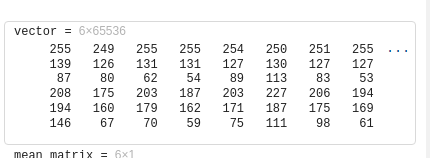
\includegraphics[width = 0.75\textwidth]{imgs/3a1.png}
    \caption{Combined image vectors}
    \label{fig:3a1}
\end{figure}

\noindent We can see the vector is of the expected size, $6x65536$. We then find that the calculated mean matrix is:

\begin{equation}
    \begin{bmatrix}   
        108.8263 \\
        110.2227 \\
        108.4957 \\
        157.1799 \\
        141.9874 \\
        109.6162 \\
    \end{bmatrix}
\end{equation}

\noindent ...and our resulting $C_x$ comes to:

\begin{equation}
    C_x = 10^3 *
    \begin{bmatrix}
        1.4610 &    1.2925 &    1.1335 &   -0.3030 &    0.4125 &    1.0947 \\
        1.2925 &    1.2832 &    1.1826 &   -0.2736 &    0.4329 &    1.1341 \\
        1.1335 &    1.1826 &    1.3830 &   -0.3537 &    0.3605 &    1.3074 \\
        -0.3030 &   -0.2736 &   -0.3537 &    0.8365 &    0.3419 &   -0.3855 \\
        0.4125 &    0.4329 &    0.3605 &    0.3419 &    0.5007 &    0.3596 \\
        1.0947 &    1.1341 &    1.3074 &   -0.3855 &    0.3596 &    1.3695 \\
    \end{bmatrix}
\end{equation}

\noindent ...and our eigenvectors and values, respectively:

\begin{equation}
    \begin{bmatrix}
        0.3125 &   -0.4534 &   -0.0681 &   -0.6654 &   -0.0827 &    0.4925 \\
        -0.6413 &    0.5152 &   -0.0615 &   -0.2757 &   -0.0969 &    0.4838 \\
        0.4548 &    0.2810 &   -0.5261 &    0.4365 &    0.0457 &    0.4947 \\
        -0.2122 &   -0.2711 &   -0.4210 &    0.1286 &   -0.8179 &   -0.1367 \\
        0.3710 &    0.3267 &    0.6487 &    0.0682 &   -0.5535 &    0.1542 \\
        -0.3187 &   -0.5195 &    0.3415 &    0.5192 &    0.0795 &    0.4859 \\
    \end{bmatrix}
\end{equation}

\begin{equation}
    10^3 * 
    \begin{bmatrix}
        0.0373    &     0     &    0  &       0    &     0 &        0 \\
        0  &  0.0656    &     0     &    0    &     0   &      0 \\
        0    &     0  &  0.0914       &  0       &  0      &   0 \\
        0     &    0  &       0  &  0.4151    &     0  &       0 \\
        0      &   0   &      0   &      0   & 1.0620   &      0 \\
        0     &    0      &   0    &     0     &    0   & 5.1623 \\
    \end{bmatrix}
\end{equation}

\subsection*{B}

Here we are tasked with solving the $y$ vectors where $y = A(x-m_x)$. We must also compute $C_y = A C_x A^T$.

\noindent First, we solved for $A$:

\begin{equation}
    A = 
    \begin{bmatrix}    
        0.4925 &    0.4838 &    0.4947 &   -0.1367 &    0.1542 &    0.4859 \\
        -0.0827 &   -0.0969 &    0.0457 &   -0.8179 &   -0.5535 &    0.0795 \\
        -0.6654 &   -0.2757 &    0.4365 &    0.1286 &    0.0682 &    0.5192 \\
        -0.0681 &   -0.0615 &   -0.5261 &   -0.4210 &    0.6487 &    0.3415 \\
        -0.4534 &    0.5152 &    0.2810 &   -0.2711 &    0.3267 &   -0.5195 \\
        0.3125 &   -0.6413 &    0.4548 &   -0.2122 &    0.3710 &   -0.3187 \\
    \end{bmatrix}
\end{equation}

\noindent We can then solve for $y$ via $y=A(x-m_x)$. However, due to its size, we include a screenshot of it from MATLAB - you can get the exact value from \textit{problem\_3.mlx}.

\begin{figure}[H]
    \centering
    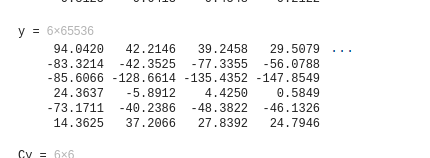
\includegraphics[width = 0.75\textwidth]{imgs/3b.png}
    \caption{$y=A(x-m_x)$}
    \label{fig:3b}
\end{figure}

\noindent And finally we can solve for $C_y$ via $C_y = A C_x A^T$:

\begin{equation}
    C_y = 10^3 *
    \begin{bmatrix}
        5.1623 &    0.0000 &    0.0000 &         0  &  -0.0000  & -0.0000 \\
        0.0000 &    1.0620 &   -0.0000 &    0.0000  &   0.0000  &  0.0000 \\
        -0.0000 &   -0.0000 &    0.4151 &    0.0000 &    0.0000 &   0.0000 \\
        -0.0000 &    0.0000 &    0.0000 &    0.0914 &   -0.0000 &  -0.0000 \\
        -0.0000 &    0.0000 &    0.0000 &   -0.0000 &    0.0656 &  -0.0000 \\
        -0.0000 &    0.0000 &    0.0000 &    0.0000 &   -0.0000 &   0.0373 \\
    \end{bmatrix}
\end{equation}

\subsection*{C}

In this section we reform the images and show them to demonstrate the principal component analysis we performed on these images, ordering them by information density.

\begin{figure}[H]
    \centering
    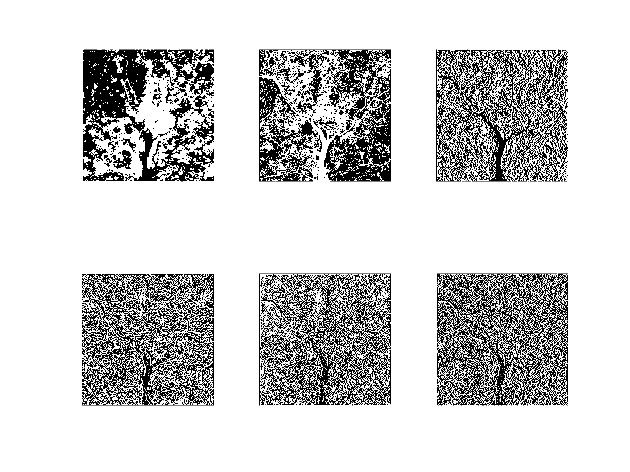
\includegraphics[width = 0.75\textwidth]{imgs/3c.jpg}
    \caption{Final images}
    \label{fig:3c}
\end{figure}


\end{document}